\section{Експериментальне дослідження моделі}

\subsection{Мета та план експериментального дослідження}\label{sec:exp-plan}

Мета моделювання за умовою задачі -- визначити, як стратегія упорядкування черги за різних
інтенсивностей надходження завдань впливає на середній час перебування завдання в системі~$W$,
середню кількість завдань у черзі~$L_q$ і середній час очікування в черзі~$W_q$. Ці три
характеристики, що обчислюються за формулами~\eqref{eq:W-total}, обрано відгуками, а факторами -- дві вхідні змінні з
таблиці~\ref{tab:inputs}:
\begin{itemize}
  \item стратегія упорядкування~$s$ -- якісний фактор з пʼятьма рівнями (таблиця~\ref{tab:strategies});
  \item коефіцієнт інтенсивності надходження~$\gamma$ ($\lambda_i = \gamma\lambda_i^0$) -- кількісний
    фактор із сімома рівнями $\gamma \in \{0{,}40;\,0{,}45;\,\ldots;\,0{,}70\}$, тобто
    $\lambda_\Sigma = 0{,}33\gamma = 0{,}132\ldots0{,}231$~завд./хв.
\end{itemize}
Фактор~$\gamma$ змінює всі потоки в однаковій пропорції ($\lambda_A : \lambda_B : \lambda_C =
0{,}2 : 0{,}07 : 0{,}06$); це обмеження дослідження, і вплив зміни лише потоку~C перевірено
окремою серією (підрозділ~\ref{sec:exp-results}). Решта параметрів незмінні
(таблиця~\ref{tab:params}): $\mu_A = 0{,}25$, $\mu_B = 0{,}2$, $\mu_C = 0{,}1$~завд./хв, $M = 2$,
$v_A = v_B = 1$, $v_C = 2$.

Експериментувати можна лише з відгуками, які з часом стабілізуються~\cite{stetsenko-kursova}.
За умови задачі ($\gamma = 1$, $\rho^0 = 1{,}175 > 1$) це не так: середня довжина черги зростає
пропорційно часу моделювання за будь-якої стратегії (рисунок~\ref{fig:exp-unstable}) і за
$t = 1{,}99\cdot10^5$~хв досягає 2296--2305~завдань для стратегій 1--2 (накопичуються завдання~C) і
8847--10\,723~завдань для стратегій 3--5 (накопичуються A і~B). Тому дослідження проведено в
області стійкості.

\begin{figure}
  \centering
  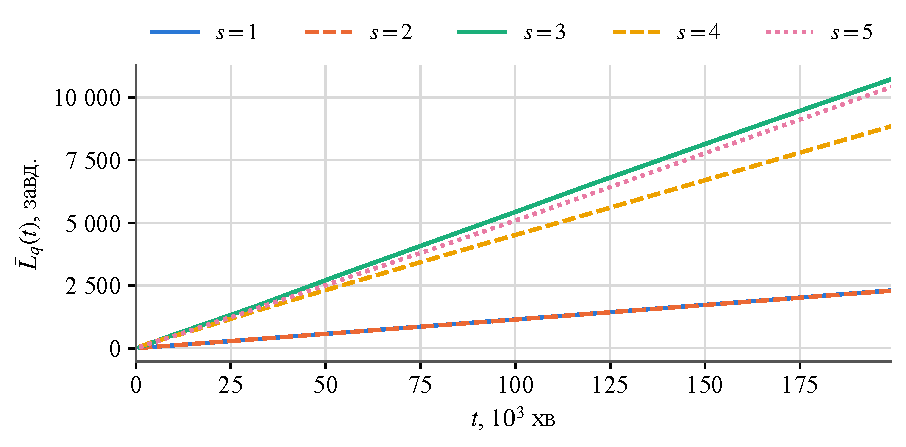
\includegraphics{media/exp-unstable}
  \caption{Середня кількість завдань у черзі на інтервалі $[0;\,t]$ за інтенсивностей з умови
    задачі ($\gamma = 1$, $\lambda_\Sigma = 0{,}33$~завд./хв, середнє за 5~прогонами)}
  \label{fig:exp-unstable}
\end{figure}

Умова $\gamma < 0{,}85$ з формули~\eqref{eq:rho} лише необхідна, тому фактичну межу визначено
прогонами за $\gamma = 0{,}75$ і~0,8 (таблиця~\ref{tab:exp-boundary}). За $\gamma = 0{,}75$ усі
стратегії стійкі: середня черга від часу не залежить, а $U = \rho = 0{,}88$. За $\gamma = 0{,}8$
($\rho = 0{,}94$) черга стратегій 1--2 зростає пропорційно часу, а $U < \rho$: завдання~C з
найнижчим пріоритетом стартує лише тоді, коли вільні обидві одиниці памʼяті й немає завдань A
і~B, а поки воно чекає, вивільнена одиниця простоює, і ці втрати перевищують запас
$1 - \rho = 0{,}06$. У стратегіях 3--5 простій обмежено резервуванням (4~\% памʼяті), і черга
стабілізується.

% Згенеровано experiments/analysis.py — не редагувати вручну
\begin{kpitable}{|c|r|r|r|r|r|r|r|}{Середня кількість завдань у черзі $\bar L_q$ на інтервалі $[0;\,t]$, завд., (5~прогонів, $t$ -- у хв) і коефіцієнт використання памʼяті $U$ (10~прогонів, $T_{\text{мод}} = 3{,}5\cdot10^6$~хв, $T_{\text{п}} = 2\cdot10^4$~хв) за рівнів $\gamma$ понад план експерименту\label{tab:exp-boundary}}
  { & \multicolumn{3}{c|}{\textbf{$\gamma = 0{,}75$ ($\lambda_\Sigma = 0{,}2475$~завд./хв)}} & \multicolumn{4}{c|}{\textbf{$\gamma = 0{,}80$ ($\lambda_\Sigma = 0{,}264$~завд./хв)}} \\ \cline{2-8}
  \textbf{$s$} & \textbf{$t = 2\cdot10^6$} & \textbf{$t = 8\cdot10^6$} & \textbf{$U$} & \textbf{$t = 2\cdot10^6$} & \textbf{$t = 4\cdot10^6$} & \textbf{$t = 8\cdot10^6$} & \textbf{$U$}}
  1 & 11,8 & 11,6 & 0,881 & 796,5 & 1\,721,8 & 3\,675,4 & 0,930 \\ \hline
  2 & 11,5 & 11,3 & 0,882 & 989,9 & 1\,701,6 & 3\,125,5 & 0,932 \\ \hline
  3 & 27,7 & 28,5 & 0,882 & 156,0 & 139,5 & 137,0 & 0,940 \\ \hline
  4 & 25,0 & 24,6 & 0,880 & 111,1 & 103,1 & 106,4 & 0,940 \\ \hline
  5 & 28,3 & 29,4 & 0,882 & 153,3 & 151,1 & 147,8 & 0,940 \\ \hline
\end{kpitable}


План обмежено рівнем $\gamma = 0{,}7$ ($\rho = 0{,}82$), щоб усі стратегії досліджувати на всіх
рівнях за однакових умов: за $\gamma = 0{,}8$ відгуки стратегій 1--2 не стабілізуються, а за
$\gamma = 0{,}75$ для стратегії~1 критерій збіжності (підрозділ~\ref{sec:exp-warmup}) вимагає
$6{,}2\cdot10^6$~хв -- майже вдвічі більше за прийнятий час моделювання. За нижньої межі
$\gamma = 0{,}4$ ($\rho = 0{,}47$) черги майже не утворюються. Метод дослідження обрано за
характером фактора~\cite{stetsenko-kursova}: вплив якісного фактора~$s$ перевірено дисперсійним
аналізом, а залежність відгуків від кількісного фактора~$\gamma$ описано рівняннями регресії.
Дані для обох методів дає повний план $5 \times 7$ з повторними прогонами.

Серії прогонів виконує клас \texttt{ExperimentRunner} із
записом результатів у файли CSV. Seed кожного прогону обчислюється за номером серії, точки плану
й прогону, тож прогони незалежні (і виконуються паралельно), а повторний запуск дає ті самі
результати:
\codeinput[firstline=232, lastline=234, gobble=4]{../sim/src/main/java/ua/kpi/km/b14/experiment/ExperimentRunner.java}
Статистичну обробку і таблиці розділу з файлів CSV виконує скрипт \texttt{analysis.py}
(SciPy~\cite{scipy}); лістинги -- у додатку~В.

\subsection{Перехідний період і час моделювання}\label{sec:exp-warmup}

Імітація починається з порожньої системи, тож відгуки на початку прогону занижені; їх
виключено зі статистики, яку збирають від моменту $T_{\text{п}}$ (таблиця~\ref{tab:kernel-mods}).
Тривалість перехідного періоду визначено за поточною довжиною черги $L_q^*(t)$, усередненою за
ансамблем із 50~прогонів у найбільш навантаженій точці $\gamma = 0{,}7$
(рисунок~\ref{fig:exp-warmup}, ковзне середнє за 2000~хв): вона виходить на сталий рівень за
$(2\ldots5)\cdot10^3$~хв. Оскільки помилка в більший бік не погіршує точності~\cite{stetsenko-kursova},
прийнято $T_{\text{п}} = 2\cdot10^4$~хв -- щонайменше з чотирикратним запасом, що становить лише 0,6~\% $T_{\text{мод}}$.

\begin{figure}
  \centering
  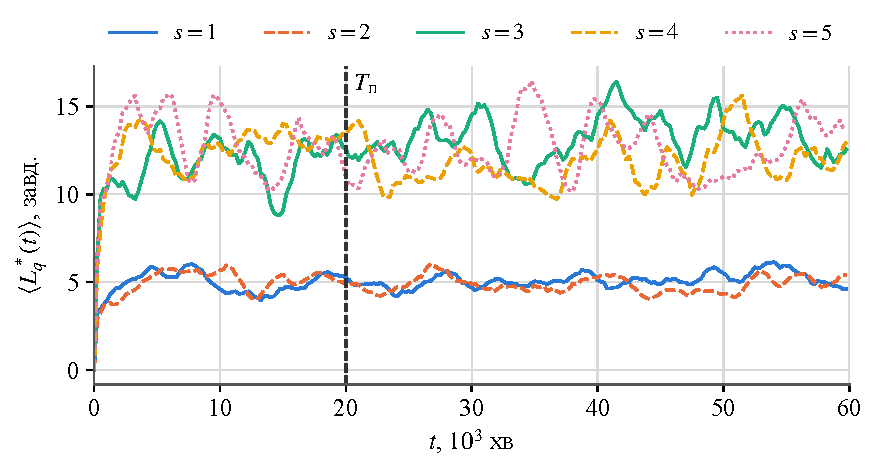
\includegraphics{media/exp-warmup}
  \caption{Поточна кількість завдань у черзі, усереднена за 50~прогонами ($\gamma = 0{,}7$)}
  \label{fig:exp-warmup}
\end{figure}

Час моделювання визначено за критерієм посібника~\cite{stetsenko-kursova}: це момент~$T$, після
якого середні значення відгуку на $[0;\,t]$, обчислені за формулою~\eqref{eq:time-means}, у пробних прогонах
відрізняються менше ніж на задану точність:
\begin{equation}\label{eq:criterion}
  T:\ \forall t \ge T,\ \forall i, j\quad \left|\bar y_i(t) - \bar y_j(t)\right| < \varepsilon,
\end{equation}
де $\bar y_i(t)$ -- середнє відгуку в $i$-му прогоні на $[0;\,t]$, $\varepsilon = 0{,}1\bar y$ --
задана точність (10~\% сталого значення).

Для кожної стратегії за $\gamma = 0{,}4$ і~0,7 виконано по 5~прогонів тривалістю
$5\cdot10^6$~хв (середні записано кожні $2{,}5\cdot10^4$~хв); значення~$T$ наведено в
таблиці~\ref{tab:exp-criterion}, приклад траєкторій -- на рисунку~\ref{fig:exp-criterion}: середні
окремих прогонів сходяться до одного рівня, тобто відгуки з часом стабілізуються. Що більше
навантаження, то довше відгуки збігаються (за $\gamma = 0{,}4$ достатньо $T \le 5{,}5\cdot10^5$~хв, за
$\gamma = 0{,}7$ потрібно до $3{,}3\cdot10^6$~хв), бо довгі черги повільно «забувають» свій стан;
найповільніше збігається~$L_q$, а $W$ містить сталу складову (час виконання) і збігається швидше. Для всіх точок плану прийнято $T_{\text{мод}} = 3{,}5\cdot10^6$~хв, що задовольняє
критерій~\eqref{eq:criterion} і в найгіршій точці ($T = 3{,}3\cdot10^6$~хв); статистику збирають на інтервалі
$[2\cdot10^4;\,3{,}5\cdot10^6]$~хв. Такий прогін за $\gamma = 0{,}7$ (близько
$8\cdot10^5$ надходжень) триває менше секунди.

% Згенеровано experiments/analysis.py — не редагувати вручну
\begin{kpitable}{|c|r|r|r|r|r|r|}{Найменший час моделювання за критерієм~\eqref{eq:criterion} ($\varepsilon = 10$~\% сталого значення, 5 прогонів), $10^6$~хв\label{tab:exp-criterion}}
  { & \multicolumn{3}{c|}{\textbf{$\gamma = 0{,}4$}} & \multicolumn{3}{c|}{\textbf{$\gamma = 0{,}7$}} \\ \cline{2-7}
  \textbf{$s$} & \textbf{$W$} & \textbf{$L_q$} & \textbf{$W_q$} & \textbf{$W$} & \textbf{$L_q$} & \textbf{$W_q$}}
  1 & 0,05 & 0,55 & 0,55 & 1,62 & 3,30 & 3,27 \\ \hline
  2 & 0,03 & 0,23 & 0,07 & 1,98 & 2,85 & 2,60 \\ \hline
  3 & 0,15 & 0,53 & 0,53 & 0,90 & 1,10 & 1,07 \\ \hline
  4 & 0,28 & 0,35 & 0,35 & 0,78 & 3,20 & 1,07 \\ \hline
  5 & 0,12 & 0,17 & 0,17 & 2,65 & 2,80 & 2,80 \\ \hline
\end{kpitable}


\begin{figure}
  \centering
  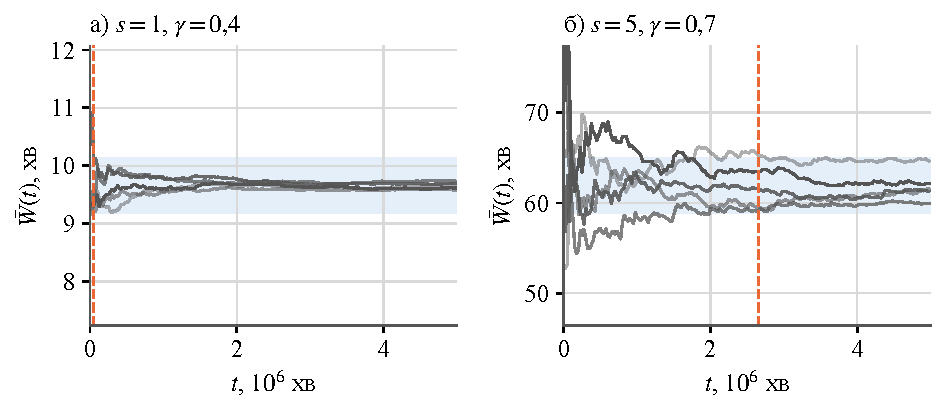
\includegraphics{media/exp-criterion}
  \caption{Середній час перебування на інтервалі $[0;\,t]$ у пʼяти прогонах ($T_{\text{п}} = 0$;
    смуга -- $\bar y \pm \varepsilon/2$, $\varepsilon = 10$~\%; штрихова лінія -- момент~$T$
    за критерієм~\eqref{eq:criterion})}
  \label{fig:exp-criterion}
\end{figure}

\subsection{Кількість прогонів і точність результатів}\label{sec:exp-runs}

Результат експерименту -- середнє відгуку за $p$ незалежними прогонами. Розкид оцінено
серією по 100~прогонів кожної стратегії за $\gamma = 0{,}7$, де він найбільший.
Центральну граничну теорему для визначення~$p$ можна застосувати лише за розподілу відгуку,
близького до нормального~\cite{stetsenko-kursova}; нормальність перевірено за критерієм згоди $\chi^2$~\cite{stetsenko-modeling} (10~рівноймовірних
інтервалів, 7~ступенів вільності, $\chi^2_{\text{кр}} = 14{,}07$ за рівня значущості 0,05).

Для стратегій 2--5 гіпотезу про нормальний закон не відхилено ($\chi^2 = 1{,}8\ldots14{,}0$), а
для стратегії~1 відхилено за всіма трьома відгуками ($\chi^2 = 14{,}8\ldots16{,}6$,
таблиця~\ref{tab:exp-pilot}; гістограма на рисунку~\ref{fig:exp-hist},~а несиметрична й має
кілька вершин). Отже, нормальність відгуку гарантувати не можна, і кількість прогонів визначено
за наслідком нерівності Чебишова~\cite{stetsenko-kursova}:
\begin{equation}\label{eq:chebyshev}
  p = \frac{\sigma^2}{\varepsilon^2\,(1-\beta)},
\end{equation}
де $\sigma$ -- стандартне відхилення відгуку в серії, $\varepsilon = 0{,}02\bar y$ --
задана точність результату (2~\% середнього), $\beta = 0{,}95$ -- довірча ймовірність.

\begin{figure}
  \centering
  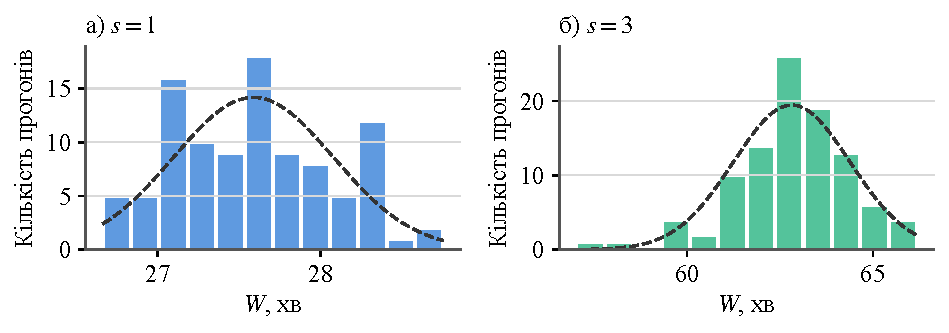
\includegraphics{media/exp-hist}
  \caption{Гістограми середнього часу перебування за 100~прогонами ($\gamma = 0{,}7$,
    $T_{\text{мод}} = 3{,}5\cdot10^6$~хв, $T_{\text{п}} = 2\cdot10^4$~хв); штрихова лінія --
    нормальний закон з вибірковими параметрами}
  \label{fig:exp-hist}
\end{figure}

% Згенеровано experiments/analysis.py — не редагувати вручну
\begin{kpitable}{|c|r|r|r|r|r|r|r|r|r|}{Розкид відгуків, критерій $\chi^2$ і потрібна кількість прогонів ($\gamma = 0{,}7$, 100 прогонів, $T_{\text{мод}} = 3{,}5\cdot10^6$~хв, $T_{\text{п}} = 2\cdot10^4$~хв, $\varepsilon = 2$~\% середнього, $\beta = 0{,}95$, $\chi^2_{\text{кр}} = 14{,}07$)\label{tab:exp-pilot}}
  { & \multicolumn{3}{c|}{\textbf{$\sigma/\bar y$, \%}} & \multicolumn{3}{c|}{\textbf{$\chi^2$}} & \multicolumn{3}{c|}{\textbf{$p$ за~\eqref{eq:chebyshev}}} \\ \cline{2-10}
  \textbf{$s$} & \textbf{$W$} & \textbf{$L_q$} & \textbf{$W_q$} & \textbf{$W$} & \textbf{$L_q$} & \textbf{$W_q$} & \textbf{$W$} & \textbf{$L_q$} & \textbf{$W_q$}}
  1 & 1,8 & 2,2 & 2,2 & 16,6 & 16,4 & 14,8 & 16 & 25 & 24 \\ \hline
  2 & 1,8 & 2,2 & 2,2 & 9,8 & 10,6 & 14,0 & 16 & 25 & 24 \\ \hline
  3 & 2,5 & 2,8 & 2,7 & 6,2 & 5,0 & 5,8 & 32 & 39 & 37 \\ \hline
  4 & 2,2 & 2,5 & 2,5 & 7,8 & 6,4 & 6,6 & 26 & 32 & 31 \\ \hline
  5 & 2,9 & 3,2 & 3,2 & 2,6 & 3,8 & 1,8 & 43 & 52 & 50 \\ \hline
\end{kpitable}


Найбільшу кількість прогонів -- 52 -- потребує $L_q$ для стратегії~5 (за центральною граничною
теоремою було б не більше 10), тому прийнято $p = 60$ прогонів у кожній точці плану. За менших
$\gamma$ розкид менший: за результатами факторного експерименту стандартне відхилення відгуку між
прогонами становить 0,4--2,8~\% середнього, точність, гарантована
нерівністю Чебишова для 60~прогонів, $\varepsilon = \sigma/\sqrt{p(1-\beta)}$, не гірша за 1,63~\%
середнього в усіх 35~точках, а половина довірчого інтервалу за розподілом Стьюдента -- не
більша за 0,73~\%.

Точності $\varepsilon = 10$~\% у критерії~\eqref{eq:criterion} і 2~\% у
формулі~\eqref{eq:chebyshev} мають різне призначення: перша визначає тривалість прогону, за якої
його середнє перестає залежати від часу, друга -- точність результату, яку забезпечує
усереднення $p$ прогонів. За $T_{\text{мод}}$ розмах середніх пʼяти прогонів становить до 9,5~\%
($L_q$, $s = 1$, $\gamma = 0{,}7$), стандартне відхилення між прогонами серії --
1,8--3,2~\% середнього, а усереднення 60~прогонів зменшує його в $\sqrt{60} \approx 7{,}7$~раза.
З $\varepsilon = 2$~\% критерій~\eqref{eq:criterion} не виконується в межах
$5\cdot10^6$~хв у 23 з 30~випадків, і одному прогону знадобилося б близько $8\cdot10^7$~хв
(розмах середніх спадає як $1/\sqrt{t}$), тоді як 60~прогонів охоплюють у точці
$2{,}1\cdot10^8$~хв модельного часу.

\subsection{Результати факторного експерименту}\label{sec:exp-results}

Повний факторний план $5 \times 7$ за $p = 60$ містить 2100~прогонів ($1{,}3\cdot10^9$
завдань, що пройшли через систему) і виконується близько 40~с. Залежність $W$
від~$\gamma$ наведено на рисунку~\ref{fig:exp-w} (точки -- експеримент,
лінії -- рівняння регресії з підрозділу~\ref{sec:exp-regression}; довірчі інтервали менші за
маркери), залежність $L_q$ -- на рисунку~\ref{fig:exp-lq}, а $W_q$ має той самий вигляд, що й~$W$; показники за типами завдань наведено в
таблиці~\ref{tab:exp-bytype} додатка~В.

\begin{figure}
  \centering
  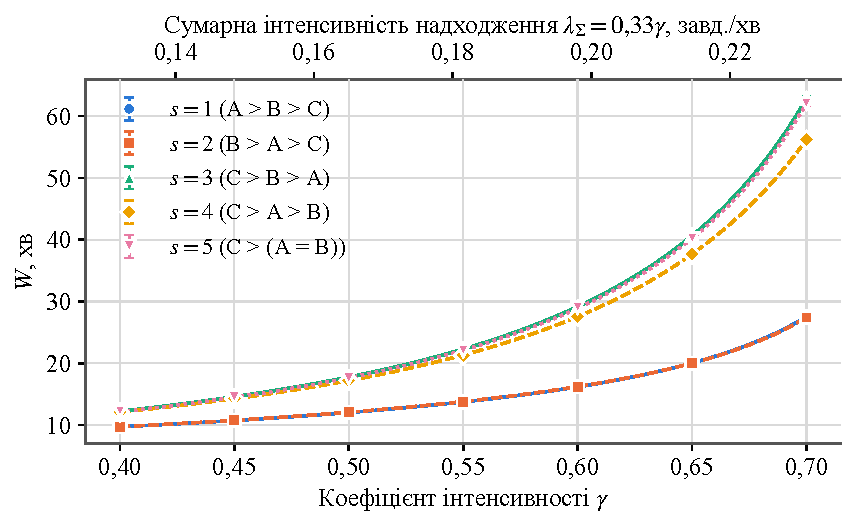
\includegraphics{media/exp-w}
  \caption{Залежність середнього часу перебування в системі від коефіцієнта інтенсивності
    ($T_{\text{мод}} = 3{,}5\cdot10^6$~хв, $T_{\text{п}} = 2\cdot10^4$~хв, 60~прогонів)}
  \label{fig:exp-w}
\end{figure}

Стратегії утворюють дві чітко розділені групи. Стратегії 1 і~2, у яких завдання~C мають
найнижчий пріоритет, дають найменші значення всіх трьох відгуків, і перевага зростає з
навантаженням: $W$ менший на 20--21~\% за $\gamma = 0{,}4$ і у 2,0--2,3 раза за $\gamma = 0{,}7$.
Короткі завдання A і~B (82~\% потоку) тут не чекають довгих завдань~C, а у стратегіях 3--5
кожне завдання~C блокує старт A і~B до звільнення всієї памʼяті (за $\gamma = 0{,}7$ через
резервування простоює 3,5~\% памʼяті). Усередині груп відмінності значно менші: стратегії 1 і~2 практично однакові, бо часи
виконання A і~B близькі, а серед 3--5 найкраща стратегія~4 (C~$>$~A~$>$~B), у якій вищий
пріоритет має найчисельніший потік коротких завдань~A. Ціна виграшу -- перерозподіл очікування
між типами: за $\gamma = 0{,}7$ завдання~C у стратегіях 1--2 перебувають у системі 99--101~хв
проти 22~хв у стратегіях 3--5, у стратегії~4 так само страждають завдання~B ($W_B = 137$~хв), а у
стратегії~3 -- завдання~A ($W_A = 88$~хв).

\begin{figure}
  \centering
  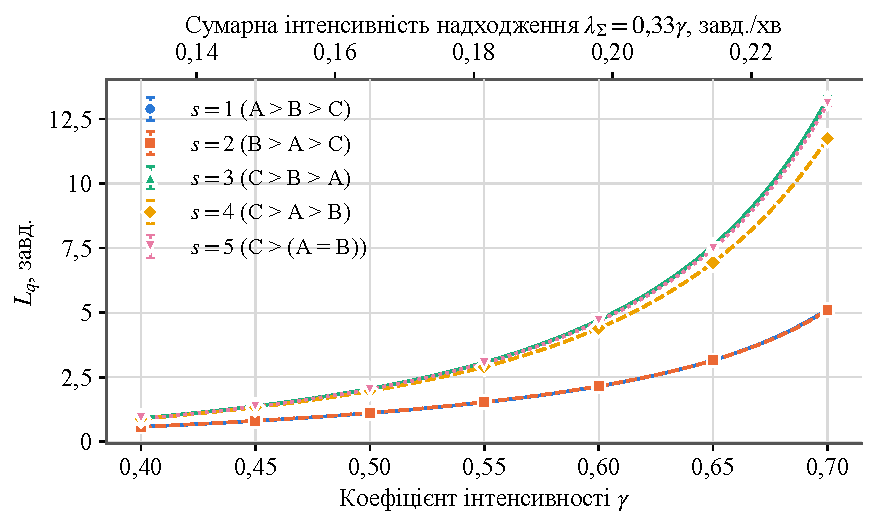
\includegraphics{media/exp-lq}
  \caption{Залежність середньої кількості завдань у черзі від коефіцієнта інтенсивності
    ($T_{\text{мод}} = 3{,}5\cdot10^6$~хв, $T_{\text{п}} = 2\cdot10^4$~хв, 60~прогонів)}
  \label{fig:exp-lq}
\end{figure}

Середні значення $W$ і $L_q$ та половини довірчих інтервалів наведено в
таблицях~\ref{tab:exp-w} і~\ref{tab:exp-lq}.

% Згенеровано experiments/analysis.py — не редагувати вручну
\begingroup\setlength{\tabcolsep}{2.5pt}
\begin{kpitable}{|c|c|r|r|r|r|r|}{Середнє значення $W$, хв, і половина довірчого інтервалу ($\beta = 0{,}95$, 60 прогонів, $T_{\text{мод}} = 3{,}5\cdot10^6$~хв, $T_{\text{п}} = 2\cdot10^4$~хв)\label{tab:exp-w}}
  {\textbf{$\gamma$} & \textbf{\begin{tabular}{@{}c@{}}$\lambda_\Sigma$,\\ завд./хв\end{tabular}} & \textbf{$s = 1$} & \textbf{$s = 2$} & \textbf{$s = 3$} & \textbf{$s = 4$} & \textbf{$s = 5$}}
  0,40 & 0,132 & 9,71$\pm$0,01 & 9,73$\pm$0,01 & 12,26$\pm$0,02 & 12,09$\pm$0,03 & 12,20$\pm$0,02 \\ \hline
  0,45 & 0,1485 & 10,73$\pm$0,02 & 10,76$\pm$0,01 & 14,56$\pm$0,03 & 14,27$\pm$0,03 & 14,48$\pm$0,04 \\ \hline
  0,50 & 0,165 & 12,02$\pm$0,02 & 12,07$\pm$0,02 & 17,75$\pm$0,05 & 17,20$\pm$0,05 & 17,57$\pm$0,05 \\ \hline
  0,55 & 0,1815 & 13,73$\pm$0,02 & 13,79$\pm$0,03 & 22,26$\pm$0,07 & 21,30$\pm$0,06 & 22,04$\pm$0,06 \\ \hline
  0,60 & 0,198 & 16,18$\pm$0,04 & 16,22$\pm$0,04 & 29,08$\pm$0,12 & 27,55$\pm$0,11 & 29,00$\pm$0,11 \\ \hline
  0,65 & 0,2145 & 20,02$\pm$0,06 & 20,01$\pm$0,06 & 40,72$\pm$0,23 & 37,67$\pm$0,16 & 40,17$\pm$0,19 \\ \hline
  0,70 & 0,231 & 27,53$\pm$0,14 & 27,40$\pm$0,13 & 62,82$\pm$0,41 & 56,20$\pm$0,28 & 62,04$\pm$0,40 \\ \hline
\end{kpitable}
\endgroup

% Згенеровано experiments/analysis.py — не редагувати вручну
\begingroup\setlength{\tabcolsep}{2.5pt}
\begin{kpitable}{|c|c|r|r|r|r|r|}{Середнє значення $L_q$, завд., і половина довірчого інтервалу ($\beta = 0{,}95$, 60 прогонів, $T_{\text{мод}} = 3{,}5\cdot10^6$~хв, $T_{\text{п}} = 2\cdot10^4$~хв)\label{tab:exp-lq}}
  {\textbf{$\gamma$} & \textbf{\begin{tabular}{@{}c@{}}$\lambda_\Sigma$,\\ завд./хв\end{tabular}} & \textbf{$s = 1$} & \textbf{$s = 2$} & \textbf{$s = 3$} & \textbf{$s = 4$} & \textbf{$s = 5$}}
  0,40 & 0,132 & 0,582$\pm$0,001 & 0,584$\pm$0,002 & 0,917$\pm$0,003 & 0,895$\pm$0,003 & 0,910$\pm$0,003 \\ \hline
  0,45 & 0,1485 & 0,806$\pm$0,003 & 0,811$\pm$0,002 & 1,374$\pm$0,005 & 1,332$\pm$0,005 & 1,362$\pm$0,005 \\ \hline
  0,50 & 0,165 & 1,109$\pm$0,003 & 1,118$\pm$0,003 & 2,053$\pm$0,008 & 1,964$\pm$0,008 & 2,025$\pm$0,008 \\ \hline
  0,55 & 0,1815 & 1,529$\pm$0,004 & 1,540$\pm$0,005 & 3,08$\pm$0,01 & 2,90$\pm$0,01 & 3,04$\pm$0,01 \\ \hline
  0,60 & 0,198 & 2,153$\pm$0,007 & 2,162$\pm$0,007 & 4,71$\pm$0,02 & 4,41$\pm$0,02 & 4,69$\pm$0,02 \\ \hline
  0,65 & 0,2145 & 3,16$\pm$0,01 & 3,15$\pm$0,01 & 7,60$\pm$0,05 & 6,94$\pm$0,03 & 7,48$\pm$0,04 \\ \hline
  0,70 & 0,231 & 5,14$\pm$0,03 & 5,11$\pm$0,03 & 13,29$\pm$0,10 & 11,75$\pm$0,06 & 13,10$\pm$0,09 \\ \hline
\end{kpitable}
\endgroup


Значення $W_q$ наведено в таблиці~\ref{tab:exp-wq}.

% Згенеровано experiments/analysis.py — не редагувати вручну
\begingroup\setlength{\tabcolsep}{2.5pt}
\begin{kpitable}{|c|c|r|r|r|r|r|}{Середнє значення $W_q$, хв, і половина довірчого інтервалу ($\beta = 0{,}95$, 60 прогонів, $T_{\text{мод}} = 3{,}5\cdot10^6$~хв, $T_{\text{п}} = 2\cdot10^4$~хв)\label{tab:exp-wq}}
  {\textbf{$\gamma$} & \textbf{\begin{tabular}{@{}c@{}}$\lambda_\Sigma$,\\ завд./хв\end{tabular}} & \textbf{$s = 1$} & \textbf{$s = 2$} & \textbf{$s = 3$} & \textbf{$s = 4$} & \textbf{$s = 5$}}
  0,40 & 0,132 & 4,41$\pm$0,01 & 4,42$\pm$0,01 & 6,95$\pm$0,02 & 6,78$\pm$0,02 & 6,90$\pm$0,02 \\ \hline
  0,45 & 0,1485 & 5,43$\pm$0,02 & 5,46$\pm$0,01 & 9,25$\pm$0,03 & 8,97$\pm$0,03 & 9,17$\pm$0,03 \\ \hline
  0,50 & 0,165 & 6,72$\pm$0,02 & 6,77$\pm$0,02 & 12,44$\pm$0,05 & 11,90$\pm$0,05 & 12,27$\pm$0,05 \\ \hline
  0,55 & 0,1815 & 8,42$\pm$0,02 & 8,48$\pm$0,03 & 16,96$\pm$0,07 & 16,00$\pm$0,06 & 16,74$\pm$0,06 \\ \hline
  0,60 & 0,198 & 10,87$\pm$0,04 & 10,92$\pm$0,04 & 23,78$\pm$0,12 & 22,25$\pm$0,10 & 23,70$\pm$0,11 \\ \hline
  0,65 & 0,2145 & 14,72$\pm$0,06 & 14,70$\pm$0,06 & 35,42$\pm$0,23 & 32,36$\pm$0,16 & 34,87$\pm$0,19 \\ \hline
  0,70 & 0,231 & 22,23$\pm$0,14 & 22,10$\pm$0,13 & 57,52$\pm$0,41 & 50,90$\pm$0,28 & 56,73$\pm$0,40 \\ \hline
\end{kpitable}
\endgroup


Вплив складу потоку перевірено серією, у якій змінюється лише потік завдань~C:
$\lambda_C = \gamma_C\cdot0{,}6\lambda_C^0$, $\gamma_C \in \{0{,}5;\,1;\,1{,}25\}$ за $\lambda_A$
і~$\lambda_B$ рівня $\gamma = 0{,}6$, для найкращих стратегій обох груп -- 1 і~4
(таблиця~\ref{tab:exp-flows}). За $\gamma_C = 1{,}25$ навантаження $\rho = 0{,}795$ не більше,
ніж у плані, тож $T_{\text{п}}$, $T_{\text{мод}}$ і $p = 60$ ті самі (точність не гірша за 1,30~\%);
точка $\gamma_C = 1$ збігається з точкою плану $\gamma = 0{,}6$ (різниця $W$ -- до 0,25~\%).

% Згенеровано experiments/analysis.py — не редагувати вручну
\begin{kpitable}{|c|c|c|c|r|r|r|r|}{Відгуки за зміни лише потоку завдань~C ($\lambda_A = 0{,}12$, $\lambda_B = 0{,}042$~завд./хв, 60~прогонів, $T_{\text{мод}} = 3{,}5\cdot10^6$~хв, $T_{\text{п}} = 2\cdot10^4$~хв)\label{tab:exp-flows}}
  {\textbf{$\gamma_C$} & \textbf{$\lambda_C$, завд./хв} & \textbf{$\rho$} & \textbf{$s$} & \textbf{$W$, хв} & \textbf{$L_q$, завд.} & \textbf{$W_q$, хв} & \textbf{$W_C$, хв}}
  0,5 & 0,018 & 0,525 & 1 & 8,81 & 0,72 & 3,97 & 22,69 \\ \hline
  0,5 & 0,018 & 0,525 & 4 & 11,14 & 1,14 & 6,31 & 15,28 \\ \hline
  1,0 & 0,036 & 0,705 & 1 & 16,16 & 2,15 & 10,86 & 45,18 \\ \hline
  1,0 & 0,036 & 0,705 & 4 & 27,62 & 4,42 & 22,32 & 19,46 \\ \hline
  1,25 & 0,045 & 0,795 & 1 & 25,96 & 4,23 & 20,45 & 80,08 \\ \hline
  1,25 & 0,045 & 0,795 & 4 & 50,45 & 9,30 & 44,94 & 22,57 \\ \hline
\end{kpitable}


Стратегія~1 лишається кращою за всіма відгуками за кожного~$\gamma_C$ ($W$ у стратегії~4 більший
у 1,26--1,94~раза), тож найкраща стратегія від співвідношення потоків не залежить. Проте
перерозподіл очікування посилюється: у стратегії~1 $W_C$ зростає в 3,5~раза, а у стратегії~4
завдання~B за $\gamma_C = 1{,}25$ перебувають у системі 112~хв.

\subsection{Дисперсійний аналіз впливу стратегії упорядкування}\label{sec:exp-anova}

Дисперсійний аналіз і перевірка рівнянь регресії припускають однаковий розкид відгуку між
прогонами в усіх точках плану, тобто відтворюваність експерименту. Її перевірено за критерієм
Кохрена~\cite{stetsenko-modeling}:
\begin{equation}\label{eq:cochran}
  G = \frac{\max_j s_j^2}{\sum_{j=1}^{N} s_j^2}, \qquad
  s_j^2 = \frac{1}{p-1}\sum_{k=1}^{p}\left(y_{jk} - \bar y_j\right)^2,
\end{equation}
де $y_{jk}$ і $\bar y_j$ -- відгук у $k$-му прогоні й середнє $j$-ї точки плану, $N = 35$ --
кількість точок. Дисперсії однорідні, якщо $G < G_{\text{кр}}$ (таблиця~\ref{tab:exp-cochran}); для $\alpha = 0{,}05$, $N = 35$ і
$p - 1 = 59$ ступенів вільності $G_{\text{кр}} = 0{,}046$.

% Згенеровано experiments/analysis.py — не редагувати вручну
\begingroup\setlength{\tabcolsep}{2pt}
\begin{kpitable}{|c|c|c|c|c|c|}{Перевірка відтворюваності за критерієм Кохрена ($\alpha = 0{,}05$; повний план -- 35~точок по 60~прогонів)\label{tab:exp-cochran}}
  {\textbf{Відгук} & \textbf{Повний план} & \textbf{$\gamma \in \{0{,}40;\,0{,}45\}$} & \textbf{$\gamma \in \{0{,}65;\,0{,}70\}$} & \textbf{Один рівень $\gamma$} & \textbf{$p = 20$}}
  $W$ & 0,271 & 0,211 & 0,304 & 0,310--0,427 & 0,305 \\ \hline
  $L_q$ & 0,294 & 0,231 & 0,318 & 0,301--0,426 & 0,326 \\ \hline
  $W_q$ & 0,273 & 0,216 & 0,305 & 0,313--0,428 & 0,308 \\ \hline
  $G_{\text{кр}}$ & 0,046 & 0,150 & 0,150 & 0,282 & 0,063 \\ \hline
\end{kpitable}
\endgroup


Для всіх відгуків $G$ у 6~разів більший за критичне значення:
дисперсії неоднорідні, найбільша з них -- у точці $s = 3$, $\gamma = 0{,}7$, а відношення
найбільшої дисперсії до найменшої сягає 1395--5428. Рекомендовані для невідтворюваного
експерименту засоби~\cite{stetsenko-modeling} -- звуження інтервалу варіювання і збільшення
кількості прогонів -- однорідності не дають: $G > G_{\text{кр}}$ і для двох сусідніх рівнів~$\gamma$,
і для кожного рівня окремо, де дисперсії пʼяти стратегій різняться в 5--15~разів, а за
$p = 10$, 20, 40, 60 критерій $G$ спадає від 0,41--0,44 лише до 0,27--0,29 (при $G_{\text{кр}}$ від
0,083 до 0,046). Отже, розкид залежить і від навантаження, і від стратегії; неоднорідність є
властивістю системи й без відмови від мети моделювання не усувається, тому далі показано, що
висновки дисперсійного аналізу від неї не залежать.

Різниця між стратегіями зростає з навантаженням (рисунки~\ref{fig:exp-w} і~\ref{fig:exp-lq}),
тому вплив стратегії перевірено однофакторним дисперсійним аналізом~\cite{stetsenko-kursova}
окремо на кожному рівні~$\gamma$. Для рівня з $q = 5$ стратегіями і $p = 60$ прогонами кожної
факторна і залишкова дисперсії
\begin{equation}\label{eq:anova-ss}
  D_F = \frac{p}{q-1}\sum_{a=1}^{q}\left(\bar y_a - \bar y\right)^2, \qquad
  D_R = \frac{1}{q(p-1)}\sum_{a=1}^{q}\sum_{k=1}^{p}\left(y_{ak} - \bar y_a\right)^2,
\end{equation}
де $y_{ak}$ -- відгук у $k$-му прогоні за стратегії~$a$, $\bar y_a$ -- середнє за стратегією,
$\bar y$ -- загальне середнє рівня. Вплив стратегії значущий, якщо відношення дисперсій~\eqref{eq:anova-ss} $F = D_F/D_R > F_{\text{кр}}$ --
квантиля розподілу Фішера рівня $1-\alpha$ зі ступенями вільності $q-1$ і $q(p-1)$,
$\alpha = 0{,}05$; результати наведено в таблиці~\ref{tab:exp-anova1}.

% Згенеровано experiments/analysis.py — не редагувати вручну
\begin{kpitable}{|c|r|r|r|c|}{Значення критерію Фішера для впливу стратегії на кожному рівні $\gamma$ ($\alpha = 0{,}05$)\label{tab:exp-anova1}}
  {\textbf{$\gamma$} & \textbf{$F$ для $W$} & \textbf{$F$ для $L_q$} & \textbf{$F$ для $W_q$} & \textbf{$F_{\text{кр}}$}}
  0,40 & 17\,215,7 & 18\,463,8 & 19\,858,6 & 2,40 \\ \hline
  0,45 & 22\,081,0 & 22\,912,8 & 24\,450,2 & 2,40 \\ \hline
  0,50 & 21\,678,4 & 21\,829,3 & 23\,052,1 & 2,40 \\ \hline
  0,55 & 29\,747,1 & 29\,559,0 & 31\,116,8 & 2,40 \\ \hline
  0,60 & 23\,047,8 & 22\,848,9 & 23\,638,6 & 2,40 \\ \hline
  0,65 & 19\,216,5 & 18\,915,3 & 19\,461,2 & 2,40 \\ \hline
  0,70 & 15\,031,4 & 14\,791,5 & 15\,130,2 & 2,40 \\ \hline
\end{kpitable}


На всіх семи рівнях і для всіх відгуків $F \ge 14\,791$ при $F_{\text{кр}} = 2{,}40$, тобто
стратегія впливає на всі три відгуки за будь-якої інтенсивності з досліджуваного діапазону.
Вплив кількісного фактора~$\gamma$ оцінено регресійним аналізом
(підрозділ~\ref{sec:exp-regression}).

Висновки стійкі до неоднорідності дисперсій: у межах одного рівня~$\gamma$ дисперсії пʼяти
стратегій різняться лише в 5--15~разів (проти 1395--5428 у плані загалом), кількість прогонів
для всіх стратегій однакова, а $F$ перевищує критичне значення понад у 6000~разів.

Значущість впливу фактора ще не означає, що різні всі його рівні, тому близькі стратегії
порівняно попарно однофакторним аналізом із двома рівнями за~$W$
($F_{\text{кр}} = 3{,}92$). Різниці між стратегіями 1 і~2 (до 0,47~\%,
на чотирьох рівнях~$\gamma$ незначуща) і між 3 і~5 (до 1,35~\%, хоча значуща на шести рівнях)
менші за задану точність 2~\%, тож ці пари практично рівноцінні. Перевага стратегії~4 над 5 і~3 значуща на
всіх рівнях ($F \ge 40{,}1$) і зростає від 0,9--1,4~\% за $\gamma = 0{,}4$ до 10,4--11,8~\% за
$\gamma = 0{,}7$.

\subsection{Регресійний аналіз залежності відгуків від інтенсивності}\label{sec:exp-regression}

Залежність відгуків від~$\gamma$ описано рівняннями регресії, лінійними за
параметрами~\cite{stetsenko-kursova}. Черга зростає пропорційно $1/(1-\rho)$, а для завдань
нижчого пріоритету -- ще швидше, тому функцією фактора обрано
$z = 1/(1 - \gamma\rho^0)$, $z \in [1{,}89;\,5{,}63]$, і за рекомендацією
посібника~\cite{stetsenko-kursova} нормалізовано її до інтервалу $[-1;\,1]$:
\begin{equation}\label{eq:normalization}
  x = \frac{z - z_0}{\Delta z}, \qquad z_0 = \frac{z_{\max} + z_{\min}}{2} = 3{,}760, \qquad
  \Delta z = \frac{z_{\max} - z_{\min}}{2} = 1{,}874.
\end{equation}
Повною моделлю прийнято поліном третього степеня від~$x$ за формулою~\eqref{eq:normalization}:
\begin{equation}\label{eq:regression}
  y = b_0 + b_1 x + b_2 x^2 + b_3 x^3.
\end{equation}
Коефіцієнти знайдено методом найменших квадратів $b = (X^{\mathrm T}X)^{-1}X^{\mathrm T}Y$ за
сімома середніми $\bar y_j$ кожної стратегії і перевірено за процедурою регресійного
аналізу~\cite{stetsenko-modeling}. Коефіцієнт $b_i$ значущий за критерієм Стьюдента, якщо
\begin{equation}\label{eq:student}
  t_i = \frac{|b_i|}{s_{b_i}} > t_{\text{кр}}, \qquad
  s_{b_i}^2 = \frac{c_{ii}\,s^2_{\text{відтв}}}{p}, \qquad
  s^2_{\text{відтв}} = \frac{1}{N}\sum_{j=1}^{N} s_j^2,
\end{equation}
де $c_{ii}$ -- діагональний елемент матриці $(X^{\mathrm T}X)^{-1}$, $s^2_{\text{відтв}}$ --
дисперсія відтворюваності (середня з дисперсій~\eqref{eq:cochran} $N = 7$ точок), $t_{\text{кр}} =
1{,}97$ -- квантиль розподілу Стьюдента рівня $1 - \alpha/2$ для $N(p-1) = 413$ ступенів вільності.
Незначущі доданки відкидають і перераховують коефіцієнти. Рівняння з $d$ коефіцієнтами
адекватне за критерієм Фішера, якщо
\begin{equation}\label{eq:fisher}
  F = \frac{s^2_{\text{ад}}}{s^2_{\text{відтв}}} < F_{\text{кр}}, \qquad
  s^2_{\text{ад}} = \frac{p}{N-d}\sum_{j=1}^{N}\left(\bar y_j - \hat y_j\right)^2,
\end{equation}
де $\hat y_j$ -- значення за рівнянням регресії, $F_{\text{кр}}$ -- квантиль розподілу Фішера
рівня $1-\alpha$ зі ступенями вільності $N - d$ і $N(p-1)$.

За формулою~\eqref{eq:student} коефіцієнти $b_0$, $b_1$, $b_2$ значущі в усіх 15~рівняннях
($t_i \ge 24{,}9$), а $b_3$ незначущий для $W$ і~$W_q$ у стратегіях 3 і~5 ($t_3 = 0{,}5\ldots1{,}1$),
тож для них доданок $x^3$ відкинуто й рівняння квадратичне; в інших 11~рівняннях
$t_3 = 2{,}4\ldots7{,}5$. За формулою~\eqref{eq:fisher} усі 15~отриманих рівнянь адекватні:
$F = 0{,}05\ldots1{,}25$ при $F_{\text{кр}} = 2{,}39$ ($d = 3$) і 2,63 ($d = 4$). Оскільки дисперсії точок неоднорідні, $s^2_{\text{відтв}}$ -- лише середня дисперсія, і висновок
про адекватність наближений; його підтверджує найбільша відносна похибка рівнянь
$\delta_{\max} = \max_j |\bar y_j - \hat y_j|/\bar y_j \le 1{,}23$~\%, менша за точність
експерименту 2~\%, та індекс кореляції
$R = \sqrt{1 - \sum_j (\bar y_j - \hat y_j)^2 / \sum_j (\bar y_j - \bar y)^2} \ge 0{,}99999$ ($\bar y$ -- середнє
з~$\bar y_j$). Коефіцієнти наведено в таблиці~\ref{tab:exp-regression} додатка~В. Простіші
види залежності, перевірені для порівняння, -- квадратичний поліном від~$z$ і поліноми від
самого~$\gamma$ -- для частини рівнянь неадекватні або мають похибку понад 2~\%.

Завдяки нормалізації коефіцієнти порівнянні ($b_0$ -- відгук у центрі діапазону,
$\gamma \approx 0{,}62$), наприклад, $W_{s=1} = 17{,}82 + 8{,}50x + 0{,}80x^2 + 0{,}42x^3$~хв і
$W_{s=4} = 31{,}88 + 22{,}40x + 2{,}27x^2 - 0{,}35x^3$~хв.
Переважає лінійний вплив~$z$ ($b_1$ у 5--12~разів більший за $|b_2|$), а відгуки стратегій
3--5 чутливіші до навантаження: $b_1$ у них у 2,5--3,0, а $b_2$ у 2,8--4,9~раза більші, ніж у 1--2.
Отже, рівняння~\eqref{eq:regression} адекватно описують залежність відгуків від інтенсивності
надходження в діапазоні $\gamma \in [0{,}4;\,0{,}7]$ і можуть замінити імітацію для наближеної
оцінки відгуків усередині цього діапазону.

\subsection{Висновки до розділу}

За інтенсивностей з умови задачі черги зростають необмежено, тому експерименти проведено за
$\gamma \in [0{,}4;\,0{,}7]$ ($T_{\text{п}} = 2\cdot10^4$~хв, $T_{\text{мод}} = 3{,}5\cdot10^6$~хв,
60~прогонів у точці, точність 2~\%); за $\gamma = 0{,}8$ першими втрачають стійкість стратегії 1--2.
Попри неоднорідність дисперсій (критерій Кохрена) дисперсійний аналіз надійно показав значущий
вплив стратегії на всі три відгуки за кожного рівня інтенсивності, причому різниця між
стратегіями зростає з~$\gamma$. Рівноцінні стратегії 1 і~2
(C -- з найнижчим пріоритетом) дають найменші значення відгуків (середній час перебування в
1,25 раза менший за $\gamma = 0{,}4$ і у 2,0--2,3 раза за $\gamma = 0{,}7$, ніж у стратегій 3--5)
коштом завдань~C; серед стратегій із пріоритетом~C найкраща стратегія~4. Зміна лише потоку~C
вибору не змінила. Залежність відгуків від інтенсивності описано адекватними рівняннями регресії
від нормалізованого фактора $1/(1-\rho)$ з похибкою до 1,2~\%.
